\documentclass{article}
\usepackage[utf8]{inputenc}
\usepackage{graphicx}
\usepackage{hyperref}
\usepackage[margin=1cm]{geometry}
 
\title{Techie_Crunch}


\begin{document}
\newpage
\begin{center}
\textbf{Capstone Project II}
\end{center}
\begin{center}
\textbf{Mobile Application Design and Development}
\end{center}
\begin{center}

\includegraphics[scale=0.7]{CALM-DOWN Logo.png}
\end{center}



\begin{center}
\textbf{Team Name :  Techie Crunch}
\end{center}
\begin{center}
\begin{tabular}{ l r }
\textbf{Team Member} & \textbf{Student ID}\\
 Roohi Singh & c0763590\\  
 Roopa Paruchuri & c0762201\\
 Kavya Devabakthuni & c0765771
\end{tabular}
\newline
\newline

\end{center}
\begin{center}
\textbf{Supervisor : Peter Sigurdson}
\end{center}
\section  * {Introduction}
CALM-DOWN is a “self-healing” tool. The application provides the users with four main tools to let them heal themselves and bring a positive change in themselves.
User can take a quiz in which user have to answer few questions and know if they are having stress and anxiety.After knowing it they can go for the music therapy as by listening to it they can calm their busy stressed mind or they can go to yoga or exercises where they can perform  either yoga asana or exercise to make their mind and body relax.Moreover they can write a journal to express their thoughts in this application.
\section{Our Vision and Concept}
\begin{abstract}
   Breathe in. Breathe out.
The state of the world is, in short, chaos. Your mental state does not have to be the same. It sounds counter intuitive,
but the very device that is delivering anxiety-inducing news could be the thing that brings you a bit of calm. Meditation apps are a welcome window into a world of gentle bells, chirping birds, and encouraging words. Beyond the peaceful imagery, the ceasing of the mind’s worry with meditation can have tremendous health benefits, easing anxiety, depression, and pain and even improving immunity.
Team Techie Crunch intends to produce an Android App named ”CALM-DOWN” that will take a quiz from user to know their anxiety, stress level and helps them to calm-down. It has some modern and ancient music to cheer-up as well as some motivational videos. It has yoga and meditation sessions which helps them to be fit and happy. It also has a journal for writing all their experiences and good things happening around them, So they can motivate others. An annual membership (45 Dollars) gives access to a short course on how to meditate, videos and stories about meditation, and instructions on how to guide others in meditation.
Our Vision is that this product will be of value to customers which helps to reveal the diamond nature of your own mind, so your appreciation of it can be more direct and intimate, and not covered up with all the stuff that keeps it from shining.
\end{abstract}
\section{Use Cases}
\begin{enumerate}
    \item \textbf{Actor : } A user who is so stressed out and don't have a stable mind and body,frequently experiencing anxiety.
    \item \textbf{Goal : } A user who wants to attain stable mind and body, who needs to be stress free and to calm mind from anxiety attacks will find this app very helpful.
     \item \textbf{Steps : }By using this a user can know anxiety level and stress level by answering few questions.User can express their thoughts so that they don't get anxiety attacks as it happens by thinking too much about something.Moreover by using the music therapy where they gets the music of ancient and modern era to calm their mind and thoughts.So, to maintain balance of mind and body user can perform yoga asana or exercise.
\end{enumerate}
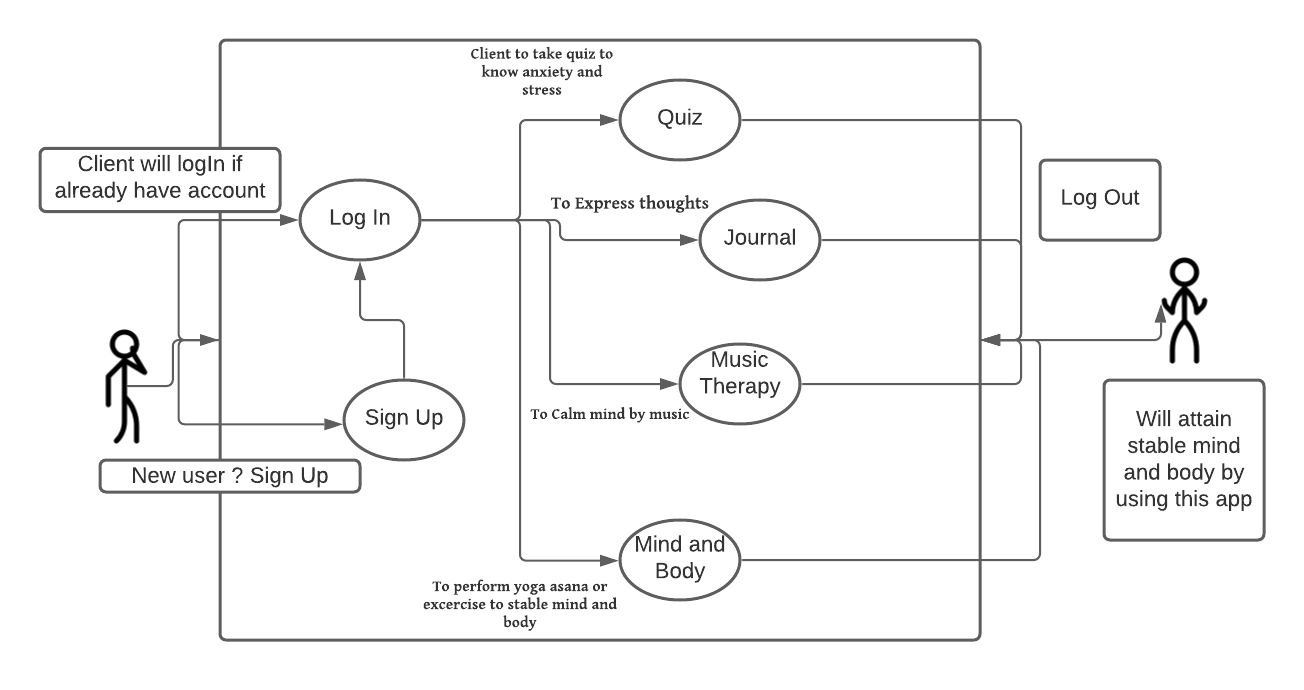
\includegraphics[scale=0.7]{UC.png}
\newline
\large{\textbf{User Story : }}
\newline
As a person I want something in the market to take me out to a world where I can be free of any stress or anxiety without having to spend an extra money for seeing a therapist so that I can live my life to the fullest and express my feelings in a way I want, simultaneously getting instant multiple helpful options to attain this.

\section{UI Prototype}
\textbf{Log In Screen Prototype :} 
\newline

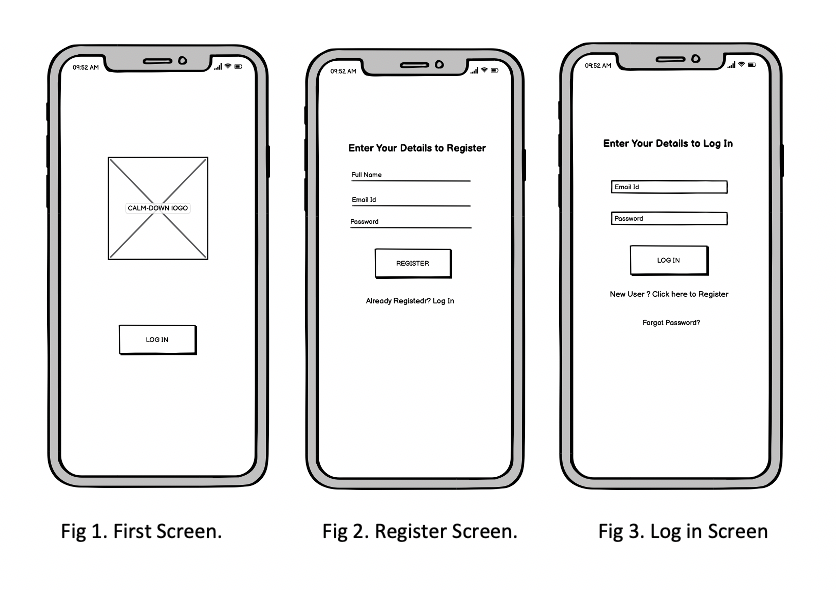
\includegraphics[scale=0.9]{loginwireframe.png}
\newline
\textbf{Main Screen Prototype :} 
\newline
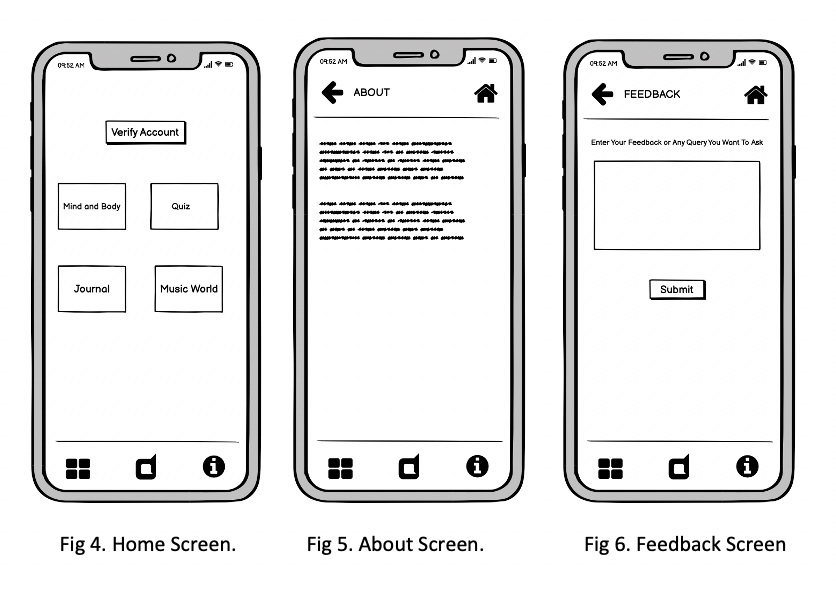
\includegraphics[scale=0.8]{mainscreenwireframe.png}
\newpage
\textbf{Monetization Screen Prototype :} 
\newline
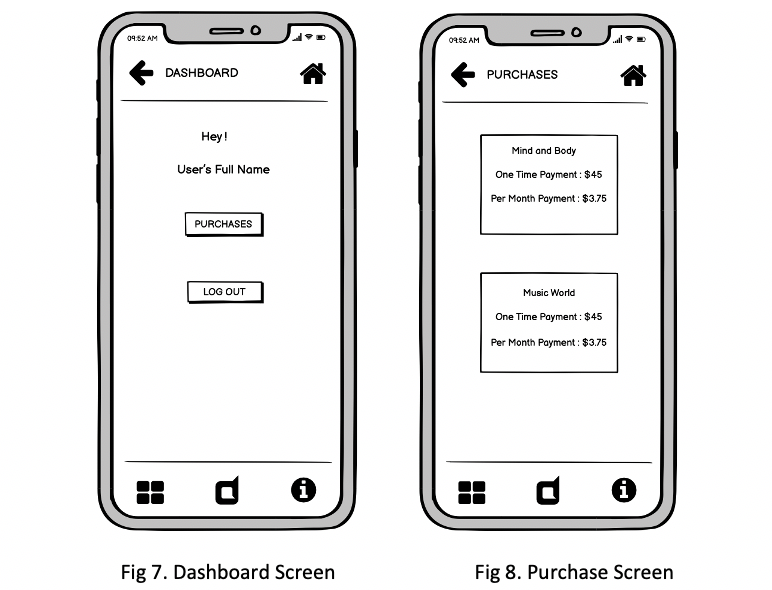
\includegraphics[scale=0.8]{monetizationwireframe.png}
\newline
\textbf{Quiz Screen Prototype :} 
\newline
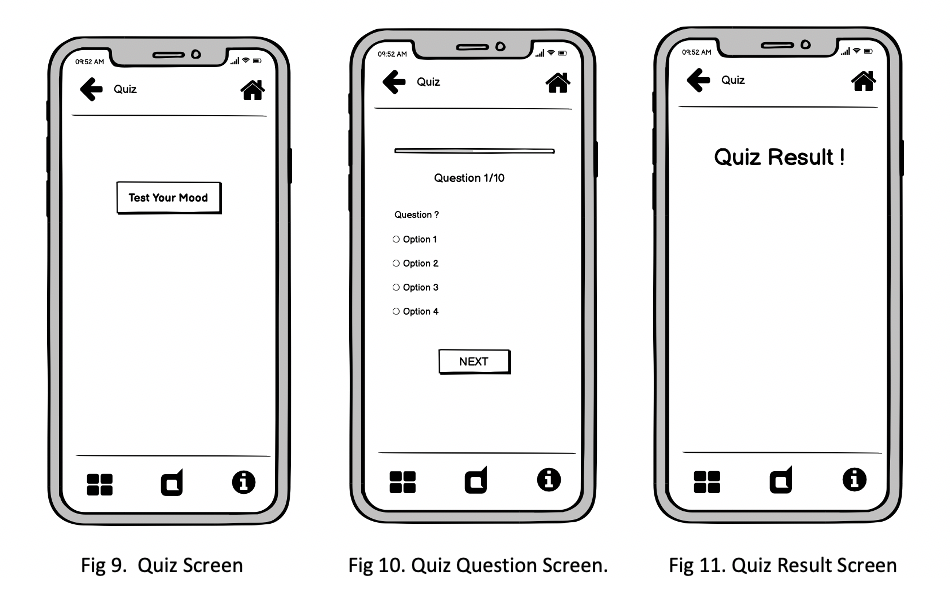
\includegraphics[scale=0.8]{quizwireframe.png}
\newpage
\textbf{Mind and Body Screen Prototype :} 
\newline
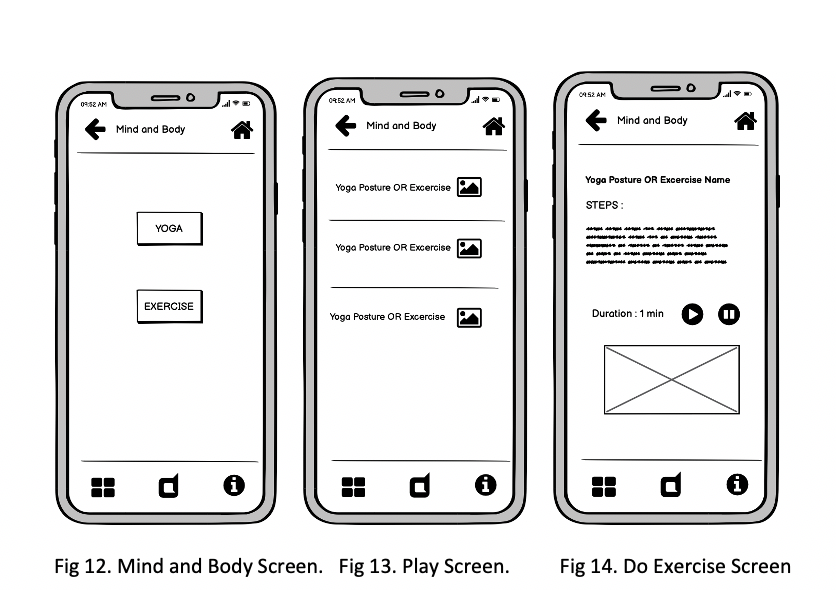
\includegraphics[scale=0.8]{mindandbodywireframe.png}
\newline
\textbf{Music World Screen Prototype :} 
\newline
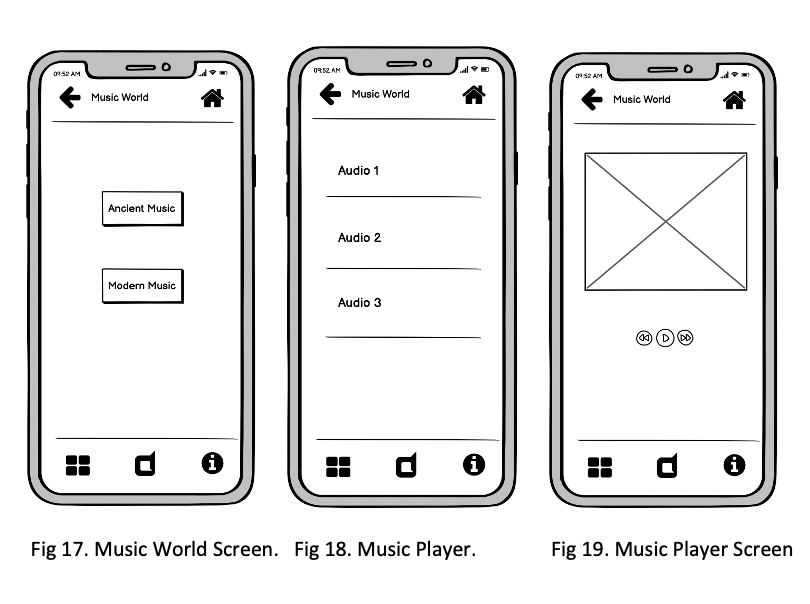
\includegraphics[scale=0.8]{musicwireframe.png}
\newpage
\textbf{Journal Screen Prototype :} 
\newline
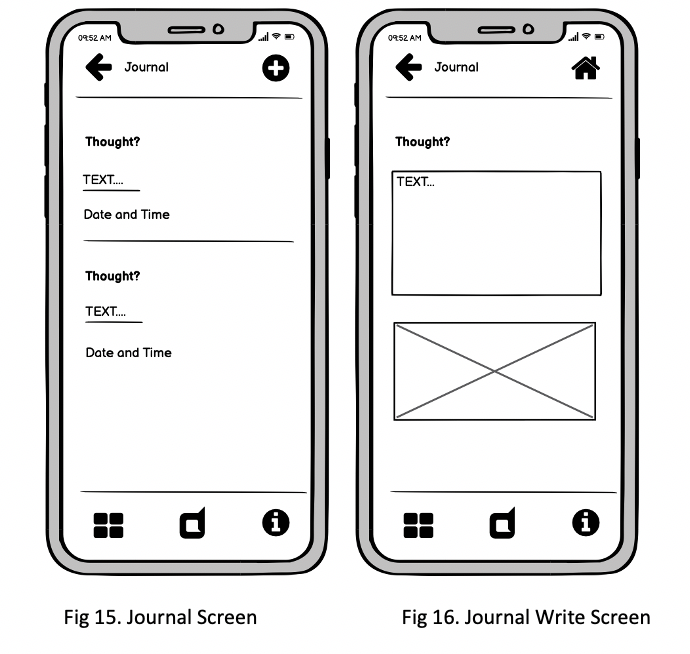
\includegraphics[scale=0.8]{journalwireframe.png}


\section{Competitive Analysis}
The competitive analysis is between three apps in market with our app.
\newline
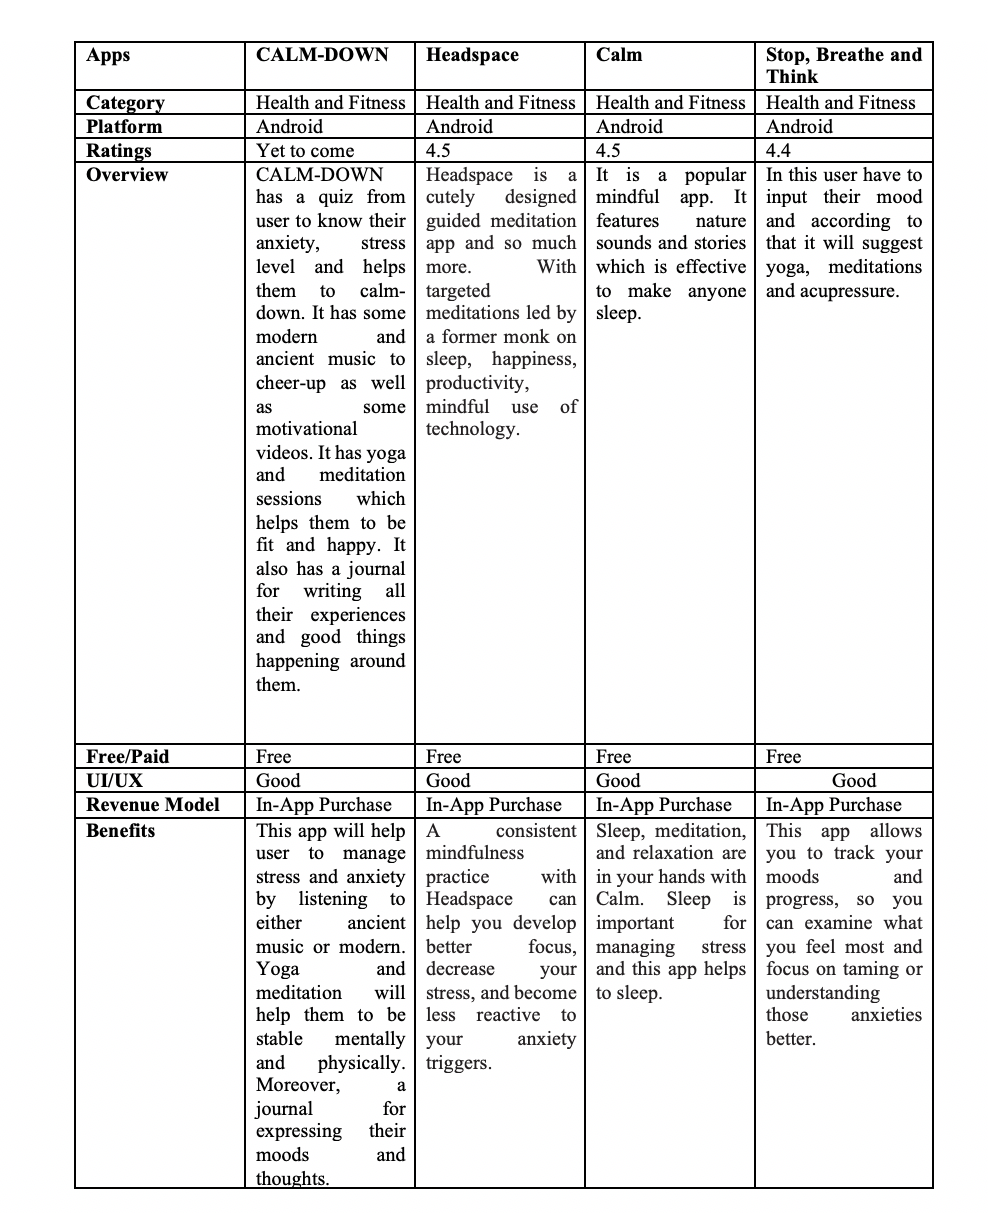
\includegraphics[scale=0.9]{CA.png}

\section{Our App Monetization Method}
\begin{enumerate}
    \item \textbf{Pricing Strategy :} In-App Purchase
    \item \textbf{Pricing Criteria :} The Quiz and Journal is free.Body exercise  and Music Therapy will be Paid. User will get the Demo of the features and the benefits it can give based on those factors they can make their decisions.
    \item \textbf{Pricing Distribution :} \begin{enumerate}
        \item Mind and Body : One time payment \$45 and per month payment \$3.75
         \item Music Therapy : One time payment \$45 and per month payment \$3.75
    \end{enumerate} 
    
\end{enumerate}
\section{Our App Timeline}
\begin{enumerate}
\item \textbf{Work Breakdown Structure in Tabular form}
\newline
\begin{center}
\begin{tabular}{ l l l  }
 \textbf{TASKS} & \textbf{START DATE}  \\
 Analysis and Planning & 7 August 2020  \\  
Wireframming & 7 August 2020 \\
UI Design & 8 August 2020 \\
UI Development & 9 August 2020 \\
Internal Testing & 11 August 2020 \\
Development & 14 August 2020 \\
User Management & 19 August 2020 \\
Testing & 20 August 2020 \\
Launch & 23 August 2020 \\
Marketing & 25 August 2020
\end{tabular}
\end{center}
\item \textbf{Gantt Chart} 
\newline
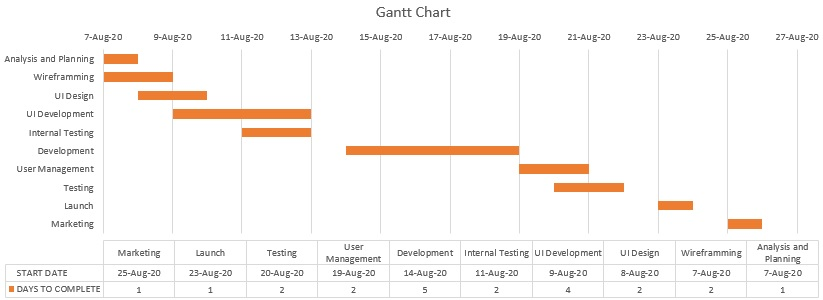
\includegraphics[scale=.7]{gantt chart photo.jpg}
\end{enumerate}


\section{Test Cases}
A TEST CASE is a set of conditions or variables under which a tester will determine whether a system under test satisfies requirements or works correctly. The process of developing test cases can also help find problems in the requirements or design of an application
\newline
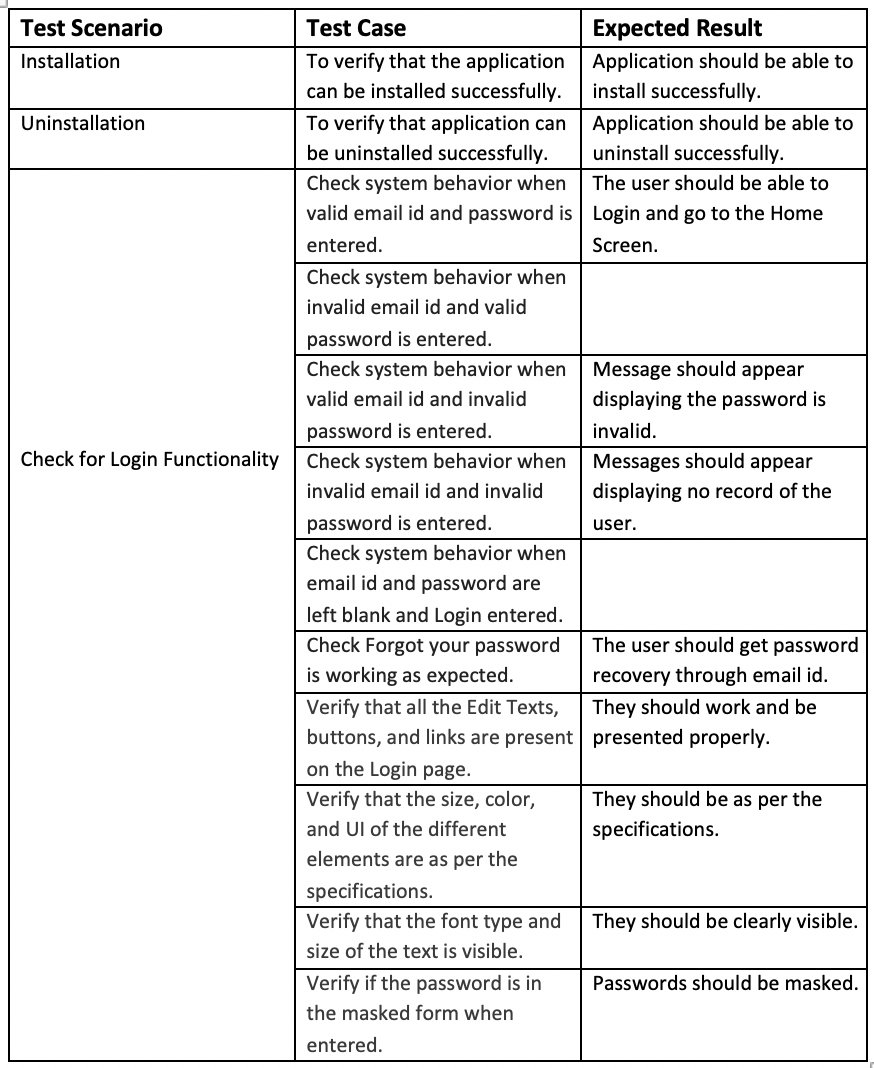
\includegraphics[scale=0.9]{testcase1.png}


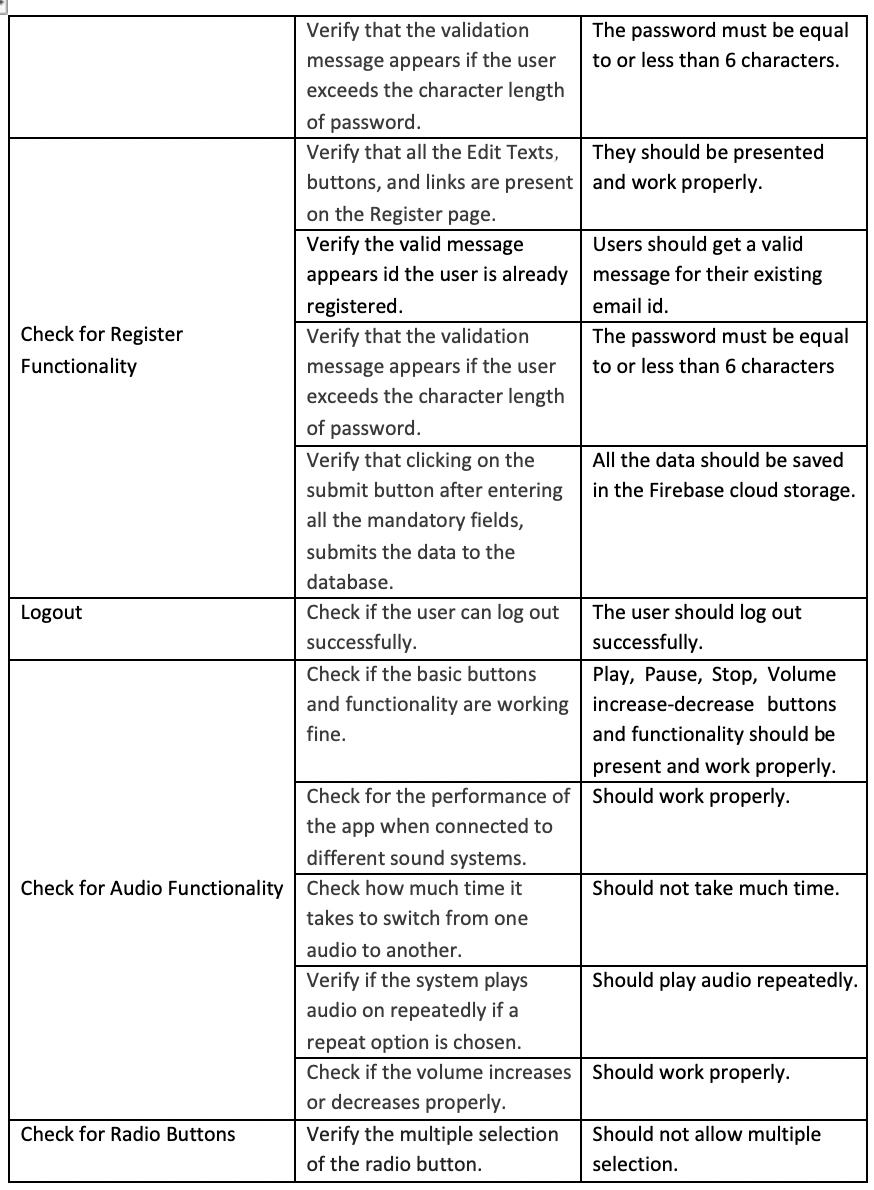
\includegraphics[scale=0.9]{testcase2.png}
\newpage
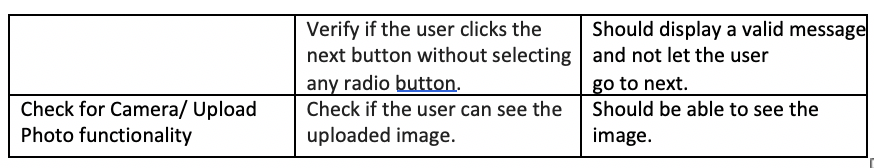
\includegraphics[scale=0.9]{testcase3.png}
\section{Our Marketing Strategy}
\begin{enumerate}
    \item \textbf{Targeted Audience :}  age 12 - any age
    \item \textbf{An App Preview Video : }  It will help to demonstrate our app’s features, functionality and UI. Instead of just screenshots, we
    will add an app preview video to our Play Store page. It’s a great marketing strategy to engage users browsing the Play Store, and help them learn more about our app.We can easily show it on our landing page, in a Facebook ad, or on YouTube as well.
    \item \textbf{Local Media : } It is more cost-effective to reach a local audience. Reach, exposure and real-world engagement is all we need right now. We will Build a genuine connection, and care about helping people in our local community. It will land us more eyeballs, an interview, or engagement from the people we seek to serve.
    \item \textbf{Optimize App  : } For Google Play Store,We have used well-researched keywords in the application name, and we will strategically place throughout our listing, so we show up when users search for those words.It will improve our app visibility and drive downloads well, because they come up at the exact moment the customer is searching for an app like ours. It’s perfect timing.
     \item \textbf{Feedback and Reviews : } More than 60 percent of users check out an app’s rating before installing the app. And users are more likely to write a review after a negative experience in the app.We will notify users of our feedback form, so they’ll know how to contact us before they run into issues.
\end{enumerate}


\section{Links}
\begin{enumerate}
    \item Google Site Link :
\url{https://sites.google.com/view/calmdownmankind}
\item Github Link : 
\url{https://github.com/RoohiSingh-GH/calmdown}
\item Latex File link : \url{https://github.com/RoohiSingh-GH/Techie_CrunchLatex}
\item Latex Link :
\url{https://github.com/RoohiSingh-GH/Techie_CrunchLatex}
\end{enumerate}



\end{document}
